% !TEX TS-program = pdflatex
% !TEX encoding = UTF-8 Unicode
\documentclass[border=0mm]{standalone}
% packages
\usepackage{tikz}
\usetikzlibrary{patterns}
\usepackage{amsmath,amssymb}
\usepackage{bm}
\usepackage{pgfplots}
\pgfplotsset{compat=1.15}
% start document
\begin{document}
% generated by ROOT (CERN)
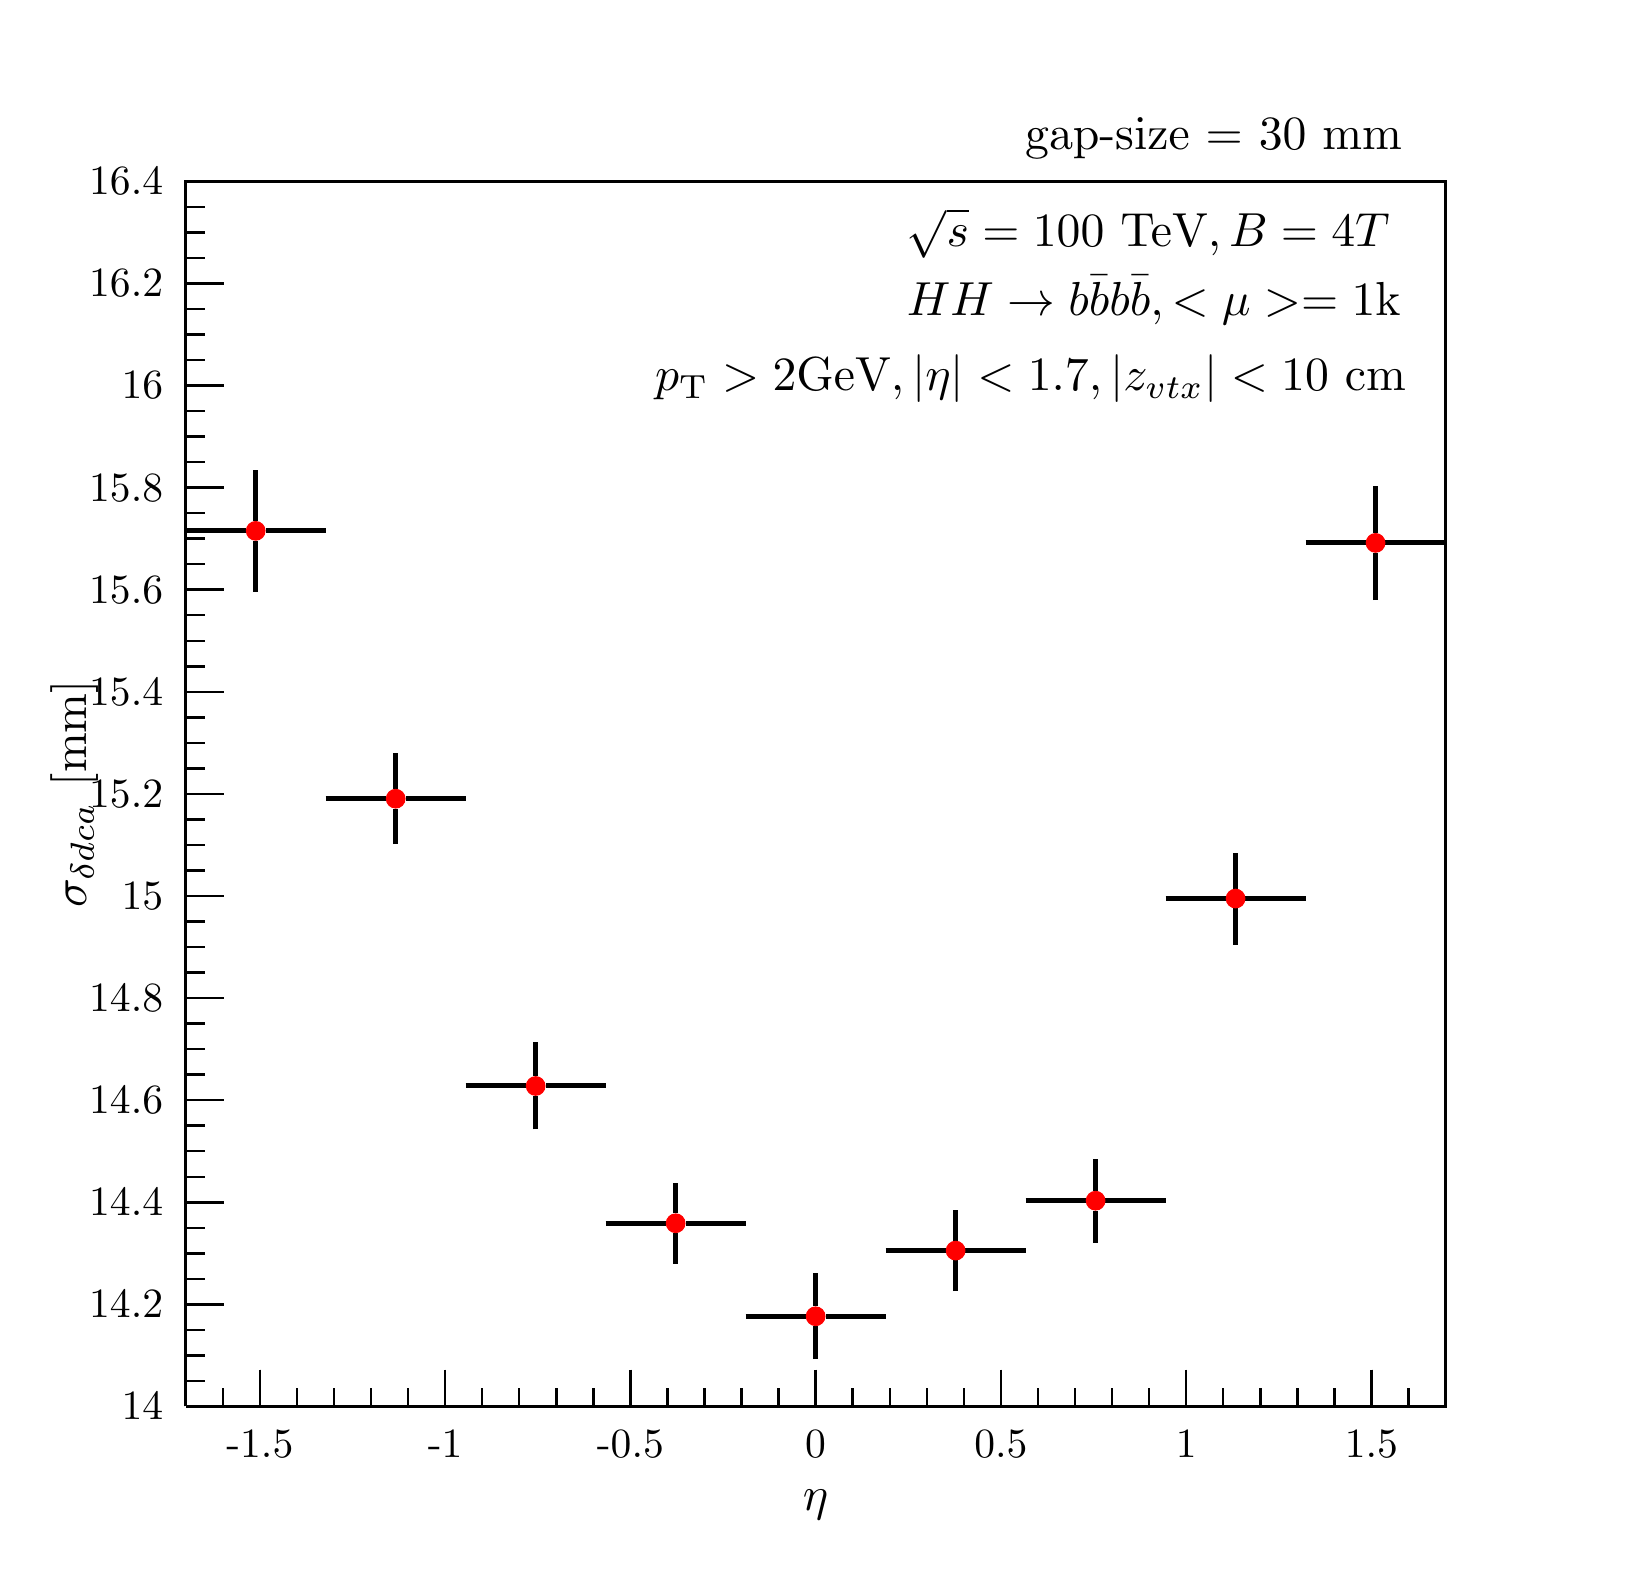
\begin{tikzpicture}
\pgfdeclareplotmark{cross} {
\pgfpathmoveto{\pgfpoint{-0.3\pgfplotmarksize}{\pgfplotmarksize}}
\pgfpathlineto{\pgfpoint{+0.3\pgfplotmarksize}{\pgfplotmarksize}}
\pgfpathlineto{\pgfpoint{+0.3\pgfplotmarksize}{0.3\pgfplotmarksize}}
\pgfpathlineto{\pgfpoint{+1\pgfplotmarksize}{0.3\pgfplotmarksize}}
\pgfpathlineto{\pgfpoint{+1\pgfplotmarksize}{-0.3\pgfplotmarksize}}
\pgfpathlineto{\pgfpoint{+0.3\pgfplotmarksize}{-0.3\pgfplotmarksize}}
\pgfpathlineto{\pgfpoint{+0.3\pgfplotmarksize}{-1.\pgfplotmarksize}}
\pgfpathlineto{\pgfpoint{-0.3\pgfplotmarksize}{-1.\pgfplotmarksize}}
\pgfpathlineto{\pgfpoint{-0.3\pgfplotmarksize}{-0.3\pgfplotmarksize}}
\pgfpathlineto{\pgfpoint{-1.\pgfplotmarksize}{-0.3\pgfplotmarksize}}
\pgfpathlineto{\pgfpoint{-1.\pgfplotmarksize}{0.3\pgfplotmarksize}}
\pgfpathlineto{\pgfpoint{-0.3\pgfplotmarksize}{0.3\pgfplotmarksize}}
\pgfpathclose
\pgfusepathqstroke
}
\pgfdeclareplotmark{cross*} {
\pgfpathmoveto{\pgfpoint{-0.3\pgfplotmarksize}{\pgfplotmarksize}}
\pgfpathlineto{\pgfpoint{+0.3\pgfplotmarksize}{\pgfplotmarksize}}
\pgfpathlineto{\pgfpoint{+0.3\pgfplotmarksize}{0.3\pgfplotmarksize}}
\pgfpathlineto{\pgfpoint{+1\pgfplotmarksize}{0.3\pgfplotmarksize}}
\pgfpathlineto{\pgfpoint{+1\pgfplotmarksize}{-0.3\pgfplotmarksize}}
\pgfpathlineto{\pgfpoint{+0.3\pgfplotmarksize}{-0.3\pgfplotmarksize}}
\pgfpathlineto{\pgfpoint{+0.3\pgfplotmarksize}{-1.\pgfplotmarksize}}
\pgfpathlineto{\pgfpoint{-0.3\pgfplotmarksize}{-1.\pgfplotmarksize}}
\pgfpathlineto{\pgfpoint{-0.3\pgfplotmarksize}{-0.3\pgfplotmarksize}}
\pgfpathlineto{\pgfpoint{-1.\pgfplotmarksize}{-0.3\pgfplotmarksize}}
\pgfpathlineto{\pgfpoint{-1.\pgfplotmarksize}{0.3\pgfplotmarksize}}
\pgfpathlineto{\pgfpoint{-0.3\pgfplotmarksize}{0.3\pgfplotmarksize}}
\pgfpathclose
\pgfusepathqfillstroke
}
\pgfdeclareplotmark{newstar} {
\pgfpathmoveto{\pgfqpoint{0pt}{\pgfplotmarksize}}
\pgfpathlineto{\pgfqpointpolar{44}{0.5\pgfplotmarksize}}
\pgfpathlineto{\pgfqpointpolar{18}{\pgfplotmarksize}}
\pgfpathlineto{\pgfqpointpolar{-20}{0.5\pgfplotmarksize}}
\pgfpathlineto{\pgfqpointpolar{-54}{\pgfplotmarksize}}
\pgfpathlineto{\pgfqpointpolar{-90}{0.5\pgfplotmarksize}}
\pgfpathlineto{\pgfqpointpolar{234}{\pgfplotmarksize}}
\pgfpathlineto{\pgfqpointpolar{198}{0.5\pgfplotmarksize}}
\pgfpathlineto{\pgfqpointpolar{162}{\pgfplotmarksize}}
\pgfpathlineto{\pgfqpointpolar{134}{0.5\pgfplotmarksize}}
\pgfpathclose
\pgfusepathqstroke
}
\pgfdeclareplotmark{newstar*} {
\pgfpathmoveto{\pgfqpoint{0pt}{\pgfplotmarksize}}
\pgfpathlineto{\pgfqpointpolar{44}{0.5\pgfplotmarksize}}
\pgfpathlineto{\pgfqpointpolar{18}{\pgfplotmarksize}}
\pgfpathlineto{\pgfqpointpolar{-20}{0.5\pgfplotmarksize}}
\pgfpathlineto{\pgfqpointpolar{-54}{\pgfplotmarksize}}
\pgfpathlineto{\pgfqpointpolar{-90}{0.5\pgfplotmarksize}}
\pgfpathlineto{\pgfqpointpolar{234}{\pgfplotmarksize}}
\pgfpathlineto{\pgfqpointpolar{198}{0.5\pgfplotmarksize}}
\pgfpathlineto{\pgfqpointpolar{162}{\pgfplotmarksize}}
\pgfpathlineto{\pgfqpointpolar{134}{0.5\pgfplotmarksize}}
\pgfpathclose
\pgfusepathqfillstroke
}
\definecolor{c}{rgb}{1,1,1};
\draw [color=c, fill=c] (0,0) rectangle (20,19.4486);
\draw [color=c, fill=c] (2,1.94486) rectangle (18,17.5038);
\definecolor{c}{rgb}{0,0,0};
\draw [c,line width=0.9] (2,1.94486) -- (2,17.5038) -- (18,17.5038) -- (18,1.94486) -- (2,1.94486);
\draw [c,line width=1.8] (2.88889,12.2914) -- (2.88889,12.9396);
\draw [c,line width=1.8] (2.88889,13.1903) -- (2.88889,13.8385);
\draw [c,line width=1.8] (2,13.0649) -- (2.76358,13.0649);
\draw [c,line width=1.8] (3.0142,13.0649) -- (3.77778,13.0649);
\definecolor{c}{rgb}{1,0,0};
\foreach \P in {(2.88889,13.0649)}{\draw[mark options={color=c,fill=c},mark size=3.363363pt,mark=*] plot coordinates {\P};}
\definecolor{c}{rgb}{0,0,0};
\draw [c,line width=1.8] (4.66667,9.08641) -- (4.66667,9.53792);
\draw [c,line width=1.8] (4.66667,9.78855) -- (4.66667,10.2401);
\draw [c,line width=1.8] (3.77778,9.66324) -- (4.54135,9.66324);
\draw [c,line width=1.8] (4.79198,9.66324) -- (5.55556,9.66324);
\definecolor{c}{rgb}{1,0,0};
\foreach \P in {(4.66667,9.66324)}{\draw[mark options={color=c,fill=c},mark size=3.363363pt,mark=*] plot coordinates {\P};}
\definecolor{c}{rgb}{0,0,0};
\draw [c,line width=1.8] (6.44444,5.46239) -- (6.44444,5.88962);
\draw [c,line width=1.8] (6.44444,6.14025) -- (6.44444,6.56748);
\draw [c,line width=1.8] (5.55556,6.01494) -- (6.31913,6.01494);
\draw [c,line width=1.8] (6.56976,6.01494) -- (7.33333,6.01494);
\definecolor{c}{rgb}{1,0,0};
\foreach \P in {(6.44444,6.01494)}{\draw[mark options={color=c,fill=c},mark size=3.363363pt,mark=*] plot coordinates {\P};}
\definecolor{c}{rgb}{0,0,0};
\draw [c,line width=1.8] (8.22222,3.75869) -- (8.22222,4.14653);
\draw [c,line width=1.8] (8.22222,4.39716) -- (8.22222,4.785);
\draw [c,line width=1.8] (7.33333,4.27184) -- (8.09691,4.27184);
\draw [c,line width=1.8] (8.34754,4.27184) -- (9.11111,4.27184);
\definecolor{c}{rgb}{1,0,0};
\foreach \P in {(8.22222,4.27184)}{\draw[mark options={color=c,fill=c},mark size=3.363363pt,mark=*] plot coordinates {\P};}
\definecolor{c}{rgb}{0,0,0};
\draw [c,line width=1.8] (10,2.54701) -- (10,2.96522);
\draw [c,line width=1.8] (10,3.21585) -- (10,3.63406);
\draw [c,line width=1.8] (9.11111,3.09054) -- (9.87469,3.09054);
\draw [c,line width=1.8] (10.1253,3.09054) -- (10.8889,3.09054);
\definecolor{c}{rgb}{1,0,0};
\foreach \P in {(10,3.09054)}{\draw[mark options={color=c,fill=c},mark size=3.363363pt,mark=*] plot coordinates {\P};}
\definecolor{c}{rgb}{0,0,0};
\draw [c,line width=1.8] (11.7778,3.41109) -- (11.7778,3.79908);
\draw [c,line width=1.8] (11.7778,4.04971) -- (11.7778,4.4377);
\draw [c,line width=1.8] (10.8889,3.9244) -- (11.6525,3.9244);
\draw [c,line width=1.8] (11.9031,3.9244) -- (12.6667,3.9244);
\definecolor{c}{rgb}{1,0,0};
\foreach \P in {(11.7778,3.9244)}{\draw[mark options={color=c,fill=c},mark size=3.363363pt,mark=*] plot coordinates {\P};}
\definecolor{c}{rgb}{0,0,0};
\draw [c,line width=1.8] (13.5556,4.02721) -- (13.5556,4.43277);
\draw [c,line width=1.8] (13.5556,4.68339) -- (13.5556,5.08895);
\draw [c,line width=1.8] (12.6667,4.55808) -- (13.4302,4.55808);
\draw [c,line width=1.8] (13.6809,4.55808) -- (14.4444,4.55808);
\definecolor{c}{rgb}{1,0,0};
\foreach \P in {(13.5556,4.55808)}{\draw[mark options={color=c,fill=c},mark size=3.363363pt,mark=*] plot coordinates {\P};}
\definecolor{c}{rgb}{0,0,0};
\draw [c,line width=1.8] (15.3333,7.81179) -- (15.3333,8.26994);
\draw [c,line width=1.8] (15.3333,8.52056) -- (15.3333,8.97871);
\draw [c,line width=1.8] (14.4444,8.39525) -- (15.208,8.39525);
\draw [c,line width=1.8] (15.4586,8.39525) -- (16.2222,8.39525);
\definecolor{c}{rgb}{1,0,0};
\foreach \P in {(15.3333,8.39525)}{\draw[mark options={color=c,fill=c},mark size=3.363363pt,mark=*] plot coordinates {\P};}
\definecolor{c}{rgb}{0,0,0};
\draw [c,line width=1.8] (17.1111,12.185) -- (17.1111,12.7866);
\draw [c,line width=1.8] (17.1111,13.0373) -- (17.1111,13.6389);
\draw [c,line width=1.8] (16.2222,12.912) -- (16.9858,12.912);
\draw [c,line width=1.8] (17.2364,12.912) -- (18,12.912);
\definecolor{c}{rgb}{1,0,0};
\foreach \P in {(17.1111,12.912)}{\draw[mark options={color=c,fill=c},mark size=3.363363pt,mark=*] plot coordinates {\P};}
\definecolor{c}{rgb}{0,0,0};
\draw [c,line width=0.9] (2,1.94486) -- (18,1.94486);
\draw [c,line width=0.9] (2.94118,2.41163) -- (2.94118,1.94486);
\draw [c,line width=0.9] (3.41176,2.17825) -- (3.41176,1.94486);
\draw [c,line width=0.9] (3.88235,2.17825) -- (3.88235,1.94486);
\draw [c,line width=0.9] (4.35294,2.17825) -- (4.35294,1.94486);
\draw [c,line width=0.9] (4.82353,2.17825) -- (4.82353,1.94486);
\draw [c,line width=0.9] (5.29412,2.41163) -- (5.29412,1.94486);
\draw [c,line width=0.9] (5.76471,2.17825) -- (5.76471,1.94486);
\draw [c,line width=0.9] (6.23529,2.17825) -- (6.23529,1.94486);
\draw [c,line width=0.9] (6.70588,2.17825) -- (6.70588,1.94486);
\draw [c,line width=0.9] (7.17647,2.17825) -- (7.17647,1.94486);
\draw [c,line width=0.9] (7.64706,2.41163) -- (7.64706,1.94486);
\draw [c,line width=0.9] (8.11765,2.17825) -- (8.11765,1.94486);
\draw [c,line width=0.9] (8.58823,2.17825) -- (8.58823,1.94486);
\draw [c,line width=0.9] (9.05882,2.17825) -- (9.05882,1.94486);
\draw [c,line width=0.9] (9.52941,2.17825) -- (9.52941,1.94486);
\draw [c,line width=0.9] (10,2.41163) -- (10,1.94486);
\draw [c,line width=0.9] (10.4706,2.17825) -- (10.4706,1.94486);
\draw [c,line width=0.9] (10.9412,2.17825) -- (10.9412,1.94486);
\draw [c,line width=0.9] (11.4118,2.17825) -- (11.4118,1.94486);
\draw [c,line width=0.9] (11.8824,2.17825) -- (11.8824,1.94486);
\draw [c,line width=0.9] (12.3529,2.41163) -- (12.3529,1.94486);
\draw [c,line width=0.9] (12.8235,2.17825) -- (12.8235,1.94486);
\draw [c,line width=0.9] (13.2941,2.17825) -- (13.2941,1.94486);
\draw [c,line width=0.9] (13.7647,2.17825) -- (13.7647,1.94486);
\draw [c,line width=0.9] (14.2353,2.17825) -- (14.2353,1.94486);
\draw [c,line width=0.9] (14.7059,2.41163) -- (14.7059,1.94486);
\draw [c,line width=0.9] (15.1765,2.17825) -- (15.1765,1.94486);
\draw [c,line width=0.9] (15.6471,2.17825) -- (15.6471,1.94486);
\draw [c,line width=0.9] (16.1176,2.17825) -- (16.1176,1.94486);
\draw [c,line width=0.9] (16.5882,2.17825) -- (16.5882,1.94486);
\draw [c,line width=0.9] (17.0588,2.41163) -- (17.0588,1.94486);
\draw [c,line width=0.9] (2.94118,2.41163) -- (2.94118,1.94486);
\draw [c,line width=0.9] (2.47059,2.17825) -- (2.47059,1.94486);
\draw [c,line width=0.9] (2,2.17825) -- (2,1.94486);
\draw [c,line width=0.9] (17.0588,2.41163) -- (17.0588,1.94486);
\draw [c,line width=0.9] (17.5294,2.17825) -- (17.5294,1.94486);
\draw [c,line width=0.9] (18,2.17825) -- (18,1.94486);
\draw [anchor=base] (2.94118,1.30306) node[scale=1.50291, color=c, rotate=0]{-1.5};
\draw [anchor=base] (5.29412,1.30306) node[scale=1.50291, color=c, rotate=0]{-1};
\draw [anchor=base] (7.64706,1.30306) node[scale=1.50291, color=c, rotate=0]{-0.5};
\draw [anchor=base] (10,1.30306) node[scale=1.50291, color=c, rotate=0]{0};
\draw [anchor=base] (12.3529,1.30306) node[scale=1.50291, color=c, rotate=0]{0.5};
\draw [anchor=base] (14.7059,1.30306) node[scale=1.50291, color=c, rotate=0]{1};
\draw [anchor=base] (17.0588,1.30306) node[scale=1.50291, color=c, rotate=0]{1.5};
\draw (10,0.700151) node[scale=1.72557, color=c, rotate=0]{$\eta$};
\draw [c,line width=0.9] (2,1.94486) -- (2,17.5038);
\draw [c,line width=0.9] (2.48,1.94486) -- (2,1.94486);
\draw [c,line width=0.9] (2.24,2.26901) -- (2,2.26901);
\draw [c,line width=0.9] (2.24,2.59315) -- (2,2.59315);
\draw [c,line width=0.9] (2.24,2.91729) -- (2,2.91729);
\draw [c,line width=0.9] (2.48,3.24144) -- (2,3.24144);
\draw [c,line width=0.9] (2.24,3.56558) -- (2,3.56558);
\draw [c,line width=0.9] (2.24,3.88972) -- (2,3.88972);
\draw [c,line width=0.9] (2.24,4.21387) -- (2,4.21387);
\draw [c,line width=0.9] (2.48,4.53801) -- (2,4.53801);
\draw [c,line width=0.9] (2.24,4.86216) -- (2,4.86216);
\draw [c,line width=0.9] (2.24,5.1863) -- (2,5.1863);
\draw [c,line width=0.9] (2.24,5.51044) -- (2,5.51044);
\draw [c,line width=0.9] (2.48,5.83459) -- (2,5.83459);
\draw [c,line width=0.9] (2.24,6.15873) -- (2,6.15873);
\draw [c,line width=0.9] (2.24,6.48287) -- (2,6.48287);
\draw [c,line width=0.9] (2.24,6.80702) -- (2,6.80702);
\draw [c,line width=0.9] (2.48,7.13116) -- (2,7.13116);
\draw [c,line width=0.9] (2.24,7.45531) -- (2,7.45531);
\draw [c,line width=0.9] (2.24,7.77945) -- (2,7.77945);
\draw [c,line width=0.9] (2.24,8.10359) -- (2,8.10359);
\draw [c,line width=0.9] (2.48,8.42774) -- (2,8.42774);
\draw [c,line width=0.9] (2.24,8.75188) -- (2,8.75188);
\draw [c,line width=0.9] (2.24,9.07602) -- (2,9.07602);
\draw [c,line width=0.9] (2.24,9.40017) -- (2,9.40017);
\draw [c,line width=0.9] (2.48,9.72431) -- (2,9.72431);
\draw [c,line width=0.9] (2.24,10.0485) -- (2,10.0485);
\draw [c,line width=0.9] (2.24,10.3726) -- (2,10.3726);
\draw [c,line width=0.9] (2.24,10.6967) -- (2,10.6967);
\draw [c,line width=0.9] (2.48,11.0209) -- (2,11.0209);
\draw [c,line width=0.9] (2.24,11.345) -- (2,11.345);
\draw [c,line width=0.9] (2.24,11.6692) -- (2,11.6692);
\draw [c,line width=0.9] (2.24,11.9933) -- (2,11.9933);
\draw [c,line width=0.9] (2.48,12.3175) -- (2,12.3175);
\draw [c,line width=0.9] (2.24,12.6416) -- (2,12.6416);
\draw [c,line width=0.9] (2.24,12.9657) -- (2,12.9657);
\draw [c,line width=0.9] (2.24,13.2899) -- (2,13.2899);
\draw [c,line width=0.9] (2.48,13.614) -- (2,13.614);
\draw [c,line width=0.9] (2.24,13.9382) -- (2,13.9382);
\draw [c,line width=0.9] (2.24,14.2623) -- (2,14.2623);
\draw [c,line width=0.9] (2.24,14.5865) -- (2,14.5865);
\draw [c,line width=0.9] (2.48,14.9106) -- (2,14.9106);
\draw [c,line width=0.9] (2.24,15.2348) -- (2,15.2348);
\draw [c,line width=0.9] (2.24,15.5589) -- (2,15.5589);
\draw [c,line width=0.9] (2.24,15.883) -- (2,15.883);
\draw [c,line width=0.9] (2.48,16.2072) -- (2,16.2072);
\draw [c,line width=0.9] (2.24,16.5313) -- (2,16.5313);
\draw [c,line width=0.9] (2.24,16.8555) -- (2,16.8555);
\draw [c,line width=0.9] (2.24,17.1796) -- (2,17.1796);
\draw [c,line width=0.9] (2.48,17.5038) -- (2,17.5038);
\draw [c,line width=0.9] (2.48,17.5038) -- (2,17.5038);
\draw [anchor= east] (1.9,1.94486) node[scale=1.50291, color=c, rotate=0]{14};
\draw [anchor= east] (1.9,3.24144) node[scale=1.50291, color=c, rotate=0]{14.2};
\draw [anchor= east] (1.9,4.53801) node[scale=1.50291, color=c, rotate=0]{14.4};
\draw [anchor= east] (1.9,5.83459) node[scale=1.50291, color=c, rotate=0]{14.6};
\draw [anchor= east] (1.9,7.13116) node[scale=1.50291, color=c, rotate=0]{14.8};
\draw [anchor= east] (1.9,8.42774) node[scale=1.50291, color=c, rotate=0]{15};
\draw [anchor= east] (1.9,9.72431) node[scale=1.50291, color=c, rotate=0]{15.2};
\draw [anchor= east] (1.9,11.0209) node[scale=1.50291, color=c, rotate=0]{15.4};
\draw [anchor= east] (1.9,12.3175) node[scale=1.50291, color=c, rotate=0]{15.6};
\draw [anchor= east] (1.9,13.614) node[scale=1.50291, color=c, rotate=0]{15.8};
\draw [anchor= east] (1.9,14.9106) node[scale=1.50291, color=c, rotate=0]{16};
\draw [anchor= east] (1.9,16.2072) node[scale=1.50291, color=c, rotate=0]{16.2};
\draw [anchor= east] (1.9,17.5038) node[scale=1.50291, color=c, rotate=0]{16.4};
\draw (0.592,9.72431) node[scale=1.72557, color=c, rotate=90]{$\sigma_{\delta dca} ~[\text{mm}]$};
\draw [anchor=base west] (10.945,16.6748) node[scale=1.72557, color=c, rotate=0]{$\sqrt{s} = 100 ~\text{TeV}, B = 4T$};
\draw [anchor=base west] (10.945,15.7996) node[scale=1.72557, color=c, rotate=0]{$HH \rightarrow b\bar{b}b\bar{b}, <\mu> = \text{1k}$};
\draw [anchor=base east] (17.7105,14.8432) node[scale=1.72557, color=c, rotate=0]{$p_{\text{T}} > 2\text{GeV}, |\eta| < 1.7, |z_{vtx}| < 10\text{~cm}$};
\draw [anchor=base west] (12.445,17.9122) node[scale=1.72557, color=c, rotate=0]{gap-size = 30 mm};
\draw [anchor=base west] (12.445,17.5232) node[scale=1.72557, color=c, rotate=0]{ };
\end{tikzpicture}
% end document
\end{document}
